\chapter{Theoretical background}
\section{Tracking}
Video tracking or object tracking in a images sequence is the process of estimating the trajectory of a moving object or various objects time by time in videos or images sequences recorded by a camera or multiple cameras. Tracking action of object can be done by continuously localizing the object with information about regions, points or features of objects in images.\\
Video tracking is widely applied in many fields: human-computer interaction, security and surveillance, traffic control. Many tracking methods have been proposed to tackle the tracking problems, namely, Kalman filter, KCF, CSRT...etc. In pedestrian tracking, the trajectories of the pedestrian are almost predicable and and the velocity is not varied to much or more generally, it can be called a dynamic linear model. Due to the predicting performance in the dynamic linear model and the simple implementation. I decided to use filter as the tracker in my project. The following section briefly describes about Kalman filter.
\pagebreak
\subsection{Kalman filter}
The Kalman filter is an algorithm allowing accurate inference in a linear dynamical system, where the state space of the latent variables is continuous and where all latent and observed variables have a Gaussian distribution.\cite{Kalman}

\begin{figure}[h!]
        \centering
        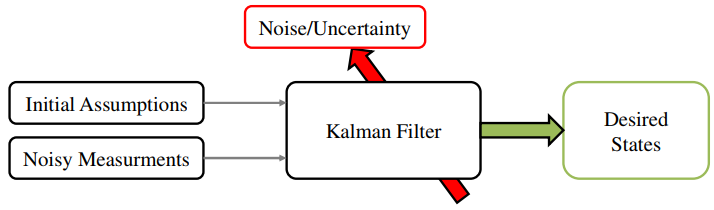
\includegraphics[width=\textwidth]{Chapters/Fig/kalman_dig.png}
        \caption{Diagram of Kalman filter}
        \label{fig:kalman_dig}
\end{figure}
Diagram of Kalman filter in fig.\ref{fig:kalman_dig} shows the goal of the filter is to take in impefect information sort out the useful parts of interest, and to reduce the uncertainty or noise.\\
The Kalman filter model assumes that the state of a system that at a time $t$ derived from the prior state at the time $t-1$ defined by the following equation:
\begin{displaymath}
 \textbf{x}_t = \textbf{F}_t \textbf{x}_{t-1} + \textbf{B}_t \textbf{x}_t + \textbf{w}_t,
\end{displaymath}
where
\begin{itemize}
    \item $\textbf{x}_t$ is the current state vector containing the parameters of interest of the system (e.g, position, velocity, accelerant..) at time t
    \item $\textbf{u}_t$ is the vector containing control inputs
    \item $\textbf{F}_t$ is the state transition matrix which applies the effect of each system state parameters at time $t-1$ on the system state at time $t$
    \item $\textbf{B}_t$ is the control input which applies the effect of each control input parameter in the control input vector $\textbf{u}_t$ on the state vector
    \item $\textbf{w}_t$ is the vector containing the process noise terms fro each parameter in the state vector.
\end{itemize}
\pagebreak
Measurements of the system is defined as follow:
\begin{displaymath}
         \textbf{z}_t = \textbf{H}_t\textbf{x}_t + \textbf{v}_t,
\end{displaymath}

where:
\begin{itemize}
    \item $\textbf{z}_t$ is the vector of measurements
    \item $\textbf{H}_t$ is the transformation matrix that maps the state vector parameters into the measurement domain
    \item $\textbf{v}_t$ is the vector containing the measurement noise terms for each observation in the measurement vector
\end{itemize}
There is no direct observation of the true state $\textbf{x}_t$ of the system, and the Kalman filter provides an algorithm to estimate $\hat{\textbf{x}}_t$ using combination of models the system and noisy measurements. Hence, for now, the terms in interest in the state vector are distributed by Gaussian probability density functions (pdfs) rather than discrete values. Gaussian pdfs come up a co-variance matrix $\textbf{P}_t$ which has the diagonal containing the variances associated with the corresponding terms in the state vector and the remaining containing the co-variance between terms in the state vectors.\\
In the prediction stage, initial state estimate, $\hat{\textbf{x}}_0$ and $\textbf{P}_0$ are applied recursively at each time step, using a loop then the current state vector is predicted from the state dynamic equation defined as:
\begin{center}
    $
        \hat{\textbf{x}}_{k|k-1} = \textbf{F}_{k-1}\hat{\textbf{x}}_{k-1} + \textbf{G}_{k-1}\textbf{u}_{k-1}
    $
\end{center}
where:
\begin{itemize}
    \item $\hat{\textbf{x}}_{k|k-1}$ is the predicted state vector
    \item $\hat{\textbf{x}}_{k}$ is the previous estimated state vector
    \item $\textbf{u}$ is the input vector
    \item $\textbf{F}$ and $\textbf{G}$ are the matrices defining the system dynamics
\end{itemize}
\pagebreak
Then we predict the state error co-variance matrix by following:
\begin{displaymath}
          \textbf{P}_{k|k-1} = \textbf{F}_{k-1}\textbf{P}_{k-1}\textbf{F}^T_{k-1} + \textbf{Q}_{k-1}
\end{displaymath}

where:
\begin{itemize}
    \item $\textbf{P}_{k|k-1}$ is the predicted state error co-variance matrix
    \item $\textbf{P}_{k-1}$ is the previous estimated state error co-variance matrix
    \item $\textbf{Q}$ is the process noise co-variance matrix.
\end{itemize}
One the predicted valued are obtained, the Kalman gain matrix, $\textbf{K}_k$ is calculated by the following function:
\begin{displaymath}
              \textbf{K}_k = \textbf{P}_{k|k-1} \textbf{H}^T_k(\textbf{H}_k\textbf{P}_{k|k-1} \textbf{H}^T_k + \textbf{R}_k)^{-1}    
\end{displaymath}

with $\textbf{R}$ is the measurement noise co-variance.\\
The measurement update equations:
\begin{itemize}
    \item The state vector is updated as:
        \begin{displaymath}
                      \hat{\textbf{x}}_k = \hat{\textbf{x}}_{k|k-1} + \textbf{K}_k(\textbf{z}_k - \textbf{H}_x\hat{\textbf{x}}_{k|k-1})
        \end{displaymath}
    \item The state error co-variance is updated by
        \begin{displaymath}
                      \textbf{P}_k = (\textbf{I} -  \textbf{K}_k\textbf{H}_k)\textbf{P}_{k|k-1}
        \end{displaymath}
\end{itemize}